%% ****** Start of file apstemplate.tex ****** %
%%
%%
%%   This file is part of the APS files in the REVTeX 4 distribution.
%%   Version 4.1r of REVTeX, August 2010
%%
%%
%%   Copyright (c) 2001, 2009, 2010 The American Physical Society.
%%
%%   See the REVTeX 4 README file for restrictions and more information.
%%
%
% This is a template for producing manuscripts for use with REVTEX 4.0
% Copy this file to another name and then work on that file.
% That way, you always have this original template file to use.
%
% Group addresses by affiliation; use superscriptaddress for long
% author lists, or if there are many overlapping affiliations.
% For Phys. Rev. appearance, change preprint to twocolumn.
% Choose pra, prb, prc, prd, pre, prl, prstab, prstper, or rmp for journal
%  Add 'draft' option to mark overfull boxes with black boxes
%  Add 'showpacs' option to make PACS codes appear
%  Add 'showkeys' option to make keywords appear
%\documentclass[aps,prl,preprint,groupedaddress]{revtex4-1}
%\documentclass[aps,prl,preprint,superscriptaddress]{revtex4-1}
%\documentclass[aps,prl,reprint,groupedaddress]{revtex4-1}
\documentclass[aps,prd,twocolumn,amsmath,amssymb,amsfont,superscriptaddress]{revtex4-1}
\usepackage{amsmath,aas_macros,xcolor,graphicx}
% You should use BibTeX and apsrev.bst for references
% Choosing a journal automatically selects the correct APS
% BibTeX style file (bst file), so only uncomment the line
% below if necessary.
%\bibliographystyle{apsrev4-1}
\bibliographystyle{h-physrev3}

\newcommand{\bs}{\boldsymbol}
\newcommand{\diff}{{\mathrm d}}
\newcommand{\Cov}{\mathsf{C}}
\newcommand{\Fish}{\mathsf{F}}
\newcommand{\Cl}{\mathcal {C}}
\newcommand{\R}{\mathcal{R}}
\newcommand{\T}{\mathcal{T}}
\newcommand{\Msun}{M_\odot}

\newcommand{\tcb}{\textcolor{blue}}
\newcommand{\tcv}{\textcolor{violet}}
\newcommand{\tcr}{\textcolor{red}}
\newcommand{\tcx}{\textcolor{teal}}


\begin{document}

% Use the \preprint command to place your local institutional report
% number in the upper righthand corner of the title page in preprint mode.
% Multiple \preprint commands are allowed.
% Use the 'preprintnumbers' class option to override journal defaults
% to display numbers if necessary
%\preprint{}

%Title of paper
\title{Neutrino Torque}

% repeat the \author .. \affiliation  etc. as needed
% \email, \thanks, \homepage, \altaffiliation all apply to the current
% author. Explanatory text should go in the []'s, actual e-mail
% address or url should go in the {}'s for \email and \homepage.
% Please use the appropriate macro foreach each type of information

% \affiliation command applies to all authors since the last
% \affiliation command. The \affiliation command should follow the
% other information
% \affiliation can be followed by \email, \homepage, \thanks as well.
\author{Hao-Ran~Yu}\email{\url{haoran@cita.utoronto.ca}}
\affiliation{Tsung-Dao Lee Institute, Shanghai Jiao Tong University, Shanghai, 200240, China}
\affiliation{Canadian Institute for Theoretical Astrophysics, University of Toronto, M5S 3H8, Ontario, Canada}
\affiliation{Department of Astronomy, Shanghai Jiao Tong University, Shanghai, 200240, China}

\author{Ue-Li~Pen}\email{\url{pen@cita.utoronto.ca}}
\affiliation{Canadian Institute for Theoretical Astrophysics, University of Toronto, M5S 3H8, Ontario, Canada}
\affiliation{Tsung-Dao Lee Institute, Shanghai Jiao Tong University, Shanghai, 200240, China}
\affiliation{Dunlap Institute for Astronomy and Astrophysics, University of Toronto, Toronto, ON M5S 3H4, Canada}
\affiliation{Canadian Institute for Advanced Research, CIFAR Program in Gravitation and Cosmology, Toronto, ON M5G 1Z8, Canada}
\affiliation{Perimeter Institute for Theoretical Physics, Waterloo, ON N2L 2Y5, Canada}

\author{Xin~Wang}\email{\url{xwang@cita.utoronto.ca}}
\affiliation{Canadian Institute for Theoretical Astrophysics, University of Toronto, M5S 3H8, Ontario, Canada}

%Collaboration name if desired (requires use of superscriptaddress
%option in \documentclass). \noaffiliation is required (may also be
%used with the \author command).
%\collaboration can be followed by \email, \homepage, \thanks as well.
%\collaboration{}
%\noaffiliation

\date{\today}

\begin{abstract}
Neutrino mass is a long-standing physics problem. The oscillation experiments and cosmological observations provide respectively lower and upper bound on their sum of mass. Using the cosmic large scale structures to constrain the neutrino mass we encounter difficulties in disentangling other degeneracy parameters and cosmic variance. Here we show that the presence of neutrino mass provides a unique contribution to spin directions of galaxies. This neutrino torque effect is unaffected by galaxy bias and cosmic variance. Recent isobaric reconstruction techniques can reliably predict the tidal shear field of neutrinos and the resulting neutrino torque can be predicted. Upcoming galaxy surveys are promising to use the neutrino torque effect to independently constrain the neutrino mass.

\end{abstract}

% insert suggested PACS numbers in braces on next line
\pacs{}
% insert suggested keywords - APS authors don't need to do this
%\keywords{}

%\maketitle must follow title, authors, abstract, \pacs, and \keywords
\maketitle

\tcb{\textit{Introduction.---}}
The flavour oscillation experiments \citep{2002PhRvL..89a1301A} discovered the mass splittings of neutrinos and placed a lower bound of the sum of their mass $M_\nu \equiv \sum_{i=1}^3 m_{\nu_i} \gtrsim$ 0.05 eV \citep{2014ChPhC..38i0001O}. 
The existence of neutrino mass has profound impacts on cosmic evolution. 
In the early Universe relativistic neutrinos modulate the matter-to-radiation ratio, and based on which the cosmic microwave background observations provide an upper bound of $M_\nu\lesssim 0.23$ eV \citep{2016A&A...594A..13P}. 
In the late Universe, neutrinos become non-relativistic, and contribute to the matter energy density $\Omega_m$. 
Unlike the majority of matter, the cold dark matter (CDM) and baryons, neutrinos maintain a high velocity dispersion, known as ``free streaming'', which reduces their gravitational collapse on small scales. A number of large scale structure (LSS) surveys 
(such as Euclid \cite{2011arXiv1110.3193L},
LSST \cite{2009arXiv0912.0201L}, eBOSS \cite{2016AJ....151...44D},
WFIRST\cite{2012SPIE.8442E..1UG}, and DESI \cite{2015AAS...22533605E}) 
are aimed to improve this upper bound using neutrino effects on LSS,
however we usually encounter difficulties in disentangling neutrino effects from other parameters, and in understanding halo bias and cosmic variance.
Recently, new nonlinear neutrinos effects on LSS are proposed to give independent measurements on neutrino mass \citep{2014PhRvL.113m1301Z,2016PhRvL.116n1301Z,2017NatAs...1E.143Y}.
Here we present a novel neutrino torque effect which modulates the angular momenta (spin) of dark matter halos, which can be measured to constrain the neutrino mass.

\tcb{\textit{Theory.---}}
In the picture of LSS formation, gravitational instability lets initial density fluctuations form dark matter halos, in which galaxies are embedded. While in these highly nonlinear structures, uncertainties of halo bias, halo merging history and baryonic mechanisms obstruct us from clearly understanding the statistics like number counts and morphologies, the spins of galaxies/halos represent a clean structure formation history in the linear Universe, which are poorly appreciated. 

The spin of a halo in Lagrangian space $\bs{j}_L\propto\int_{V_L}\bs{q}\times-\bs{\nabla}\phi\diff^3\bs{q}$ can be written in first order as $\bs{j}_I\propto\bs{\epsilon}\,\bold{I}\,\bold{T}$ \citep{1984ApJ...286...38W}, where $\phi$ is the gravitational potential, $\bs{q}$ is the Lagrangian coordinates relative to the center of mass of the protohalo in volume $V_L$, $\bold{I}=(I_{ij})=(\int_{V_L} q_i q_j \diff^3\bs{q})$ is the inertia tensor, $\bold{T}=(T_{ij})=(\partial_i\partial_j\phi)$ is the tidal shear tensor, and $\bs{\epsilon}=(\epsilon_{ijk})$ is the Levi-Civita symbol. This picture shows that the initial spin of the protohalo is generated by the misalignment between the protogalactic inertia tensor and local gravitational shear tensor, and grows at first order in the early Universe \citep{1984ApJ...286...38W}. Actually, as halos collapse, nonlinear gravity field is hard to torque small objects, and we expect the spin directions are contributed mostly in the linear regime. These can be straightforwardly tested in numerical simulations. The halo merging and baryonic feedback, usually been discussed in the halo/galaxy alignment studies, do not affect the angular momentum conservation, because connected/disconnected matter and baryonic matter in Lagrangian space are torqued by the same gravitational shear.

Neutrino density field traces CDM on large scales while smoothly distributed on small scales, because the free streaming of neutrinos makes them less susceptible to the total gravitational potential. This contributes to a predictable tidal tensor $\bold{T}_\nu(m_{\nu_i})$ depending on the their mass. Acting on the protogalactic inertia tensor $\bold{I}$ it generates an additional neutrino torque $\bs{j}^I_\nu\propto\bs{\epsilon}\,\bold{I}\,\bold{T}_\nu$. The inertia tensor $\bold{I}$ is also predictable by using the fact that protogalactic inertia $\bold{I}$ and the tidal field from CDM $\bold{T}_c$ are highly correlated in Lagrangian space \citep{2000ApJ...532L...5L,2001ApJ...555..106L}, which can be understood that $\bold{I}$ is a collection of matter to be shell-crossed to form a halo, being parallel with $\bold{T}_c$.

To optimize the cross-correlation, we construct an equivalent inertia $\bold{I}_r$ from $\bold{T}_c$, in order that $\bs{\epsilon}\,\bold{I}_r\bold{T}_\nu$ is maximumly correlated with the integrated neutrino torque 
\begin{equation}\label{eq.jnu0}
\bs{j}^I_{\nu 0}=\int a(\tau)D(\tau)\bs{\epsilon}\bold{I}(\tau)\bold{T}_\nu(\tau)\diff\tau.
\end{equation}
In the primary coordinate of $\bold{T}_c$, $\bold{T}_c$ can be eigen-decomposed as $\bold{T}_c=\sum_{i=1}^3\bold{T}^{\lambda_i}_c$ and find $\alpha_i$ such that the reconstructed
\begin{equation}\label{eq.Ir}
	\bold{I}_r=\sum_{i=1}^3\alpha_i\bold{T}^{\lambda_i}_c
\end{equation}
optimizes the cross-correlation $\mu(\bs{j}^I_{\nu 0},\bs{j}^{I_r})$, where
\begin{equation}\label{eq.jnuIr}
 	\bs{j}^{I_r}_\nu=\bs{\epsilon}\,\bold{I}_r\bold{T}_\nu
\end{equation}
is the reconstructed neutrino spin direction.

\begin{figure}
\centering
  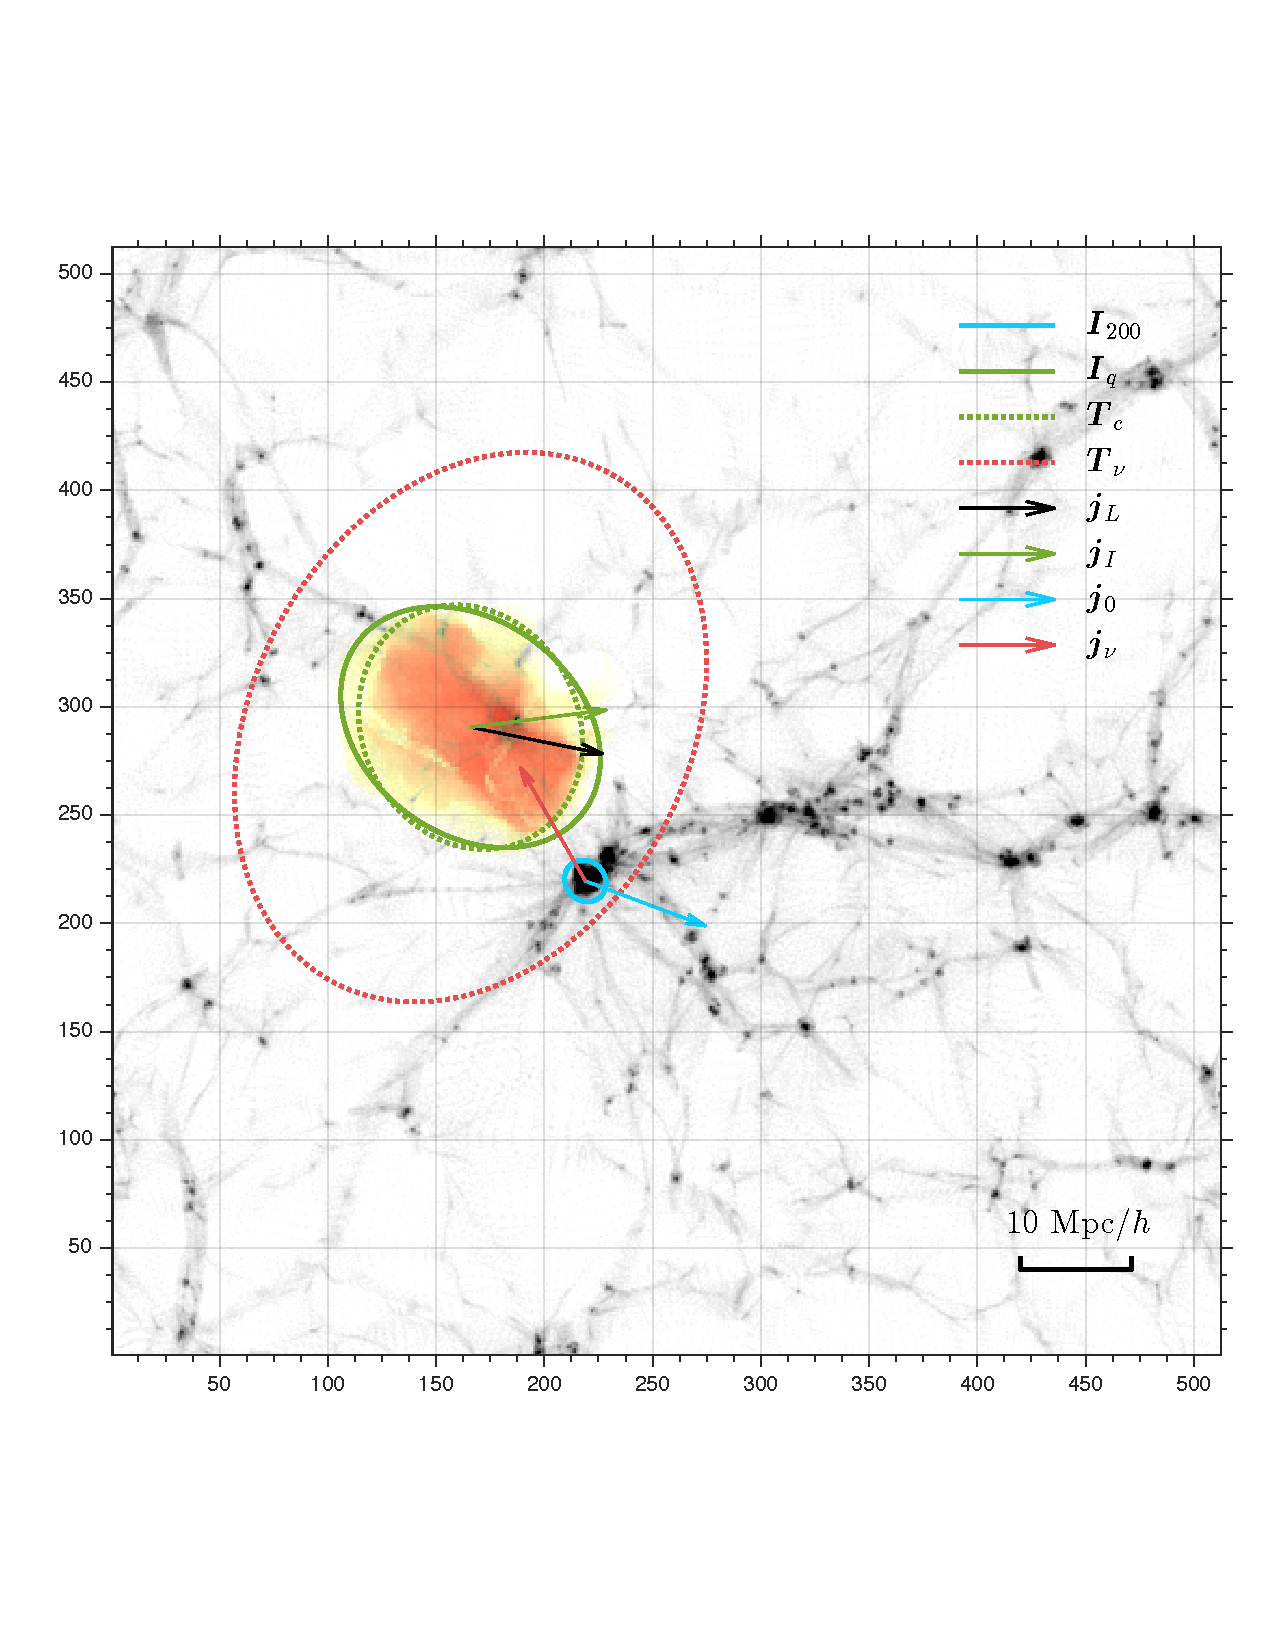
\includegraphics[width=1\linewidth]{f1}
 \caption{Illustration of the initial spin direction $\bs{j}_L$ of a protohalo region, and its tidal torque theory prediction $\bs{j}_I$ calculated by the inertia tensor $\bold{I}$ and tidal shear tensor $\bold{T}_c$. The halo at present epoch is marked with the $r_{200}$ circle with its spin direction $\bs{j}_0$, highly correlated with $\bs{j}_L$ and $\bs{j}_I$. We show that neutrino tidal torque $\bs{j}_\nu$ is generally uncorrelated with $\bs{j}_0$.}\label{fig.1}
\end{figure}


\tcb{\textit{Simulation.---}}
These correlations and coefficients are tested across a set of high-resolution $N$-body simulations \citep{2018ApJS..237...24Y}. Given any halo produced by the simulation, all the belonging particles are mapped back to Lagrangian space. The status of this definite set of particles can be traced in a resimulation, for example, their spin $\bs{j}(z)=m_p\sum\bs{x}(z)\times\bs{v}(z)$ relative to their center of mass. In Fig.\ref{fig.1} we plot (note that all quantities are projected onto the plane of this letter) the LSS from a simulation at redshift $z=0$, and mark one selected halo with its $r_{200}$ radius (within which the mean halo density is 200 times the mean matter density of the universe) and its spin direction $\bs{j}(z=0)$ (all the spin arrows are normalized to have 15 Mpc$/h$). 
We illustrate Lagrangian mapping of this halo with its protohalo's column density (the orange clouds), with its initial spin direction $\bs{j}_L$. We can see that the Lagrangian spin $\bs{j}_L$ and Eulerian spin $\bs{j}_0$ have similar directions. \tcb{Indeed, by averaging over all the halos in the simulation, we find the expectation value of the cross-correlation coefficient $\left\langle \bs{j}(z) \cdot \bs{j}_L \right\rangle$ is smoothly decreasing from unity to 0.80.} This shows that the halo spin direction is conserved from the initial state all the way to the final state of the Universe.

We next examine the tidal torque formulation. To the first order approximation, the protohalo's inertia tensor $\bold{I}$ is represented by an equivalent ellipsoid (projected as a solid ellipse in Fig.\ref{fig.1}) with its volume equals to $V_L$.
Similarly, the initial tidal shear tensor from CDM, $\bold{T}_c$, is shown the dotted green ellipsoid with same volume. The initial tidal shear from neutrinos, $\bold{T}_\nu$ is shown by the dotted red ellipsoid (8 times the volume of $V_L$, for clearity). The initial spins given by the tidal torque theory are the interplays between $\bold{I}$ and $\bold{T}_{c/\nu}$, shown in Fig.\ref{fig.1}) as $\bs{j}_I$ and $\bs{j}_\nu$. Obviously $\bs{j}_I$ has similar direction with $\bs{j}_L$ and $\bs{j}(z=0)$, where as $\bs{j}_\nu$ gives an independent direction. \tcb{From the initial condition to the end of the simulation, $\left\langle \bs{j}(z) \cdot \bs{j}_I \right\rangle$ decreases smoothly from 0.75 to 0.69. For neutrinos, the first-order tidal torque approximation gives a perfect (with cross-correlation 0.99) representation of the actual neutrino torque and it has generally less than 0.2 cross-correlation with CDM torques.} This is expected in that $\bold{T}_c$ dominates locally \tcr{(power spectrum index?)} whereas $\bold{T}_\nu$ is contributed beyond the neutrino free-streaming scale \tcr{(is this a 4-point function?)}. These two species, however, have a highly correlated contribution in structure formation. When we consider the forces that the two species exerted to the protohalo, $\bs{F}_{c/\nu}\propto\int_{V_L}\bs{\nabla}\phi_{c/\nu}\diff^3\bs{q}$, the cross-correlation between two species is as high as 0.86 \tcr{(power spectrum index?)}.

By Eq.(\ref{eq.jnu0}) we estimate the magnitude of integrated neutrino torque \tcb{$\left\langle|\bs{j}_{0\nu}|/|\bs{j}_0|\right\rangle\simeq 3\times10^{-4}$}. In particular, the effect given by the smoother distribution for neutrinos relative to CDM accounts 0.03, while the neutrino fraction $f_\nu=3.5\times 10^{-3}$ (for $M_\nu=0.05$ eV) and the backreaction from neutrinos to CDM \tcr{$\sqrt{8}$} contribute the rest.

\tcb{Measured from simulations, $(\alpha_1,\alpha_2,\alpha_3)=(-0.18,0.18,0.02)$ optimize the cross-correlation $\left\langle\bs{j}^I_{\nu 0}\cdot\bs{j}^{I_r}_\nu\right\rangle=0.19$. In this case we need $4\times 10^8$ halos to have a $1\sigma$ detection (see Appendix A)}. 

\tcb{\textit{Discussion.---}} 
We notice that the coefficients are prominently higher than \citep{2000ApJ...532L...5L}, and we investigate numerical errors that may affect the results. P3M (particle-particle particle-mesh) algorithms result in higher $\mu_L$ and $\mu_I$ compared to PM (particle-mesh), where additional tangential forces in PM violate the angular momentum conservation. Higher mass halos in a given simulation generally have slightly higher $\mu_L$ and $\mu_I$, however the correlation is enhanced greatly as we use higher mass resolutions.

\tcb{\textit{Conclusion.---}} 

% body of paper here - Use proper section commands
% References should be done using the \cite, \ref, and \label commands
%\section{}
% Put \label in argument of \section for cross-referencing
%\section{\label{}}
%\subsection{}
%\subsubsection{}

% If in two-column mode, this environment will change to single-column
% format so that long equations can be displayed. Use
% sparingly.
%\begin{widetext}
% put long equation here
%\end{widetext}

% figures should be put into the text as floats.
% Use the graphics or graphicx packages (distributed with LaTeX2e)
% and the \includegraphics macro defined in those packages.
% See the LaTeX Graphics Companion by Michel Goosens, Sebastian Rahtz,
% and Frank Mittelbach for instance.
%
% Here is an example of the general form of a figure:
% Fill in the caption in the braces of the \caption{} command. Put the label
% that you will use with \ref{} command in the braces of the \label{} command.
% Use the figure* environment if the figure should span across the
% entire page. There is no need to do explicit centering.

% \begin{figure}
% \includegraphics{}%
% \caption{\label{}}
% \end{figure}

% Surround figure environment with turnpage environment for landscape
% figure
% \begin{turnpage}
% \begin{figure}
% \includegraphics{}%
% \caption{\label{}}
% \end{figure}
% \end{turnpage}

% tables should appear as floats within the text
%
% Here is an example of the general form of a table:
% Fill in the caption in the braces of the \caption{} command. Put the label
% that you will use with \ref{} command in the braces of the \label{} command.
% Insert the column specifiers (l, r, c, d, etc.) in the empty braces of the
% \begin{tabular}{} command.
% The ruledtabular enviroment adds doubled rules to table and sets a
% reasonable default table settings.
% Use the table* environment to get a full-width table in two-column
% Add \usepackage{longtable} and the longtable (or longtable*}
% environment for nicely formatted long tables. Or use the the [H]
% placement option to break a long table (with less control than 
% in longtable).
% \begin{table}%[H] add [H] placement to break table across pages
% \caption{\label{}}
% \begin{ruledtabular}
% \begin{tabular}{}
% Lines of table here ending with \\
% \end{tabular}
% \end{ruledtabular}
% \end{table}

% Surround table environment with turnpage environment for landscape
% table
% \begin{turnpage}
% \begin{table}
% \caption{\label{}}
% \begin{ruledtabular}
% \begin{tabular}{}
% \end{tabular}
% \end{ruledtabular}
% \end{table}
% \end{turnpage}

% Specify following sections are appendices. Use \appendix* if there
% only one appendix.
\appendix
\section{How many halos do we need in 3D}
There are $N$ halos with their unit spin vector randomly distributed on a 2D sphere, $|\bs{j}|=1$ and $\left\langle \bs{j} \right\rangle =\bs{0}$. Adding an additional vector $a\hat{\bs{x}}$ ($a\ll 1$) to $\bs{j}$ and normalize we have $\bs{j}'=(\bs{j}+a\hat{\bs{x}})/|\bs{j}+a\hat{\bs{x}}|$,then we project $\bs{j}'$ onto $\hat{\bs{x}}$ and we get the signal $b=\bs{j}'\cdot\hat{\bs{x}}$. The numerical statistics are as following: $\left\langle b \right\rangle=2a/3$ and $\sigma(b)=1/\sqrt{3N}$. So, to get a $n\sigma$ detection, $N=3n^2/4a^2$ halos will be needed.

% If you have acknowledgments, this puts in the proper section head.
%\begin{acknowledgments}
% put your acknowledgments here.
%\end{acknowledgments}

% Create the reference section using BibTeX:
\bibliography{haoran_ref}

\end{document}
%
% ****** End of file apstemplate.tex ******

